\documentclass[10pt]{article}

\usepackage[a4paper,margin=0.75in]{geometry}
\usepackage{booktabs}
\usepackage{listings}
\usepackage{xcolor}
\usepackage{amsmath}
\usepackage{graphicx}
\usepackage{float}
\usepackage{hyperref}
\usepackage{caption}
\usepackage{enumitem}
\captionsetup{font=small,skip=2pt}
\setlength{\parskip}{0.3em}
\setlength{\parindent}{0pt}

% -------------------------------------------------
% Code Style
% -------------------------------------------------

\definecolor{codegreen}{rgb}{0,0.6,0}
\definecolor{codegray}{rgb}{0.5,0.5,0.5}
\definecolor{codepurple}{rgb}{0.58,0,0.82}
\definecolor{backcolour}{rgb}{0.95,0.95,0.92}

\lstdefinestyle{pythonstyle}{
backgroundcolor=\color{backcolour},
commentstyle=\color{codegreen},
keywordstyle=\color{blue},
stringstyle=\color{codepurple},
numberstyle=\tiny\color{codegray},
basicstyle=\ttfamily\small,
numbers=left,
breaklines=true,
showstringspaces=false,
tabsize=4,
language=Python
}

\lstset{style=pythonstyle}

% -------------------------------------------------
% Report Details
% -------------------------------------------------

\title{
Deep Learning Laboratory\\
Assignment \#8
}

\author{
Siddharth Narayan Mishra\\
123CS0189
}

\date{\today}

\begin{document}
\maketitle
\vspace{-1.5em}

\section*{Setup}
CIFAR-10, 12\,000 training, 2\,000 validation and 2\,000 test images (seed 42, same split for all runs), resized to 64$\times$64 and normalised, no augmentation. Cross-entropy, Adam (lr $10^{-3}$), batch 64, 10 epochs, PyTorch default initialisation reset to seed 42 before each model. Models: \textbf{Baseline} (conv 32-64-128-128-128, FC 512-256), \textbf{Exp 2} (same convs, FC 256-128), \textbf{Exp 3} (conv 16-32-64-64-64, FC 512-256). Training ran on CPU, so times are CPU seconds for the training loops only. All comparisons use validation results; the test set was evaluated once at the end. The final training accuracy and loss are measured in evaluation mode (dropout off) after epoch 10, and the generalisation gap is that training accuracy minus validation accuracy.

\begin{table}[H]
\centering
\small
\resizebox{\linewidth}{!}{%
\begin{tabular}{lrrrrrrrr}
\toprule
Model & Train acc & Val acc & Test acc & Train loss & Val loss & Gap & Params & Time (s) \\
\midrule
Baseline & 83.7\% & 63.4\% & 62.5\% & 0.506 & 1.097 & 20.3 & 4\,751\,434 & 445 \\
Exp 2: reduced classifier & 75.8\% & 61.2\% & 62.0\% & 0.703 & 1.133 & 14.6 & 2\,554\,314 & 444 \\
Exp 3: reduced width & 80.6\% & 61.3\% & 63.3\% & 0.562 & 1.153 & 19.3 & 2\,337\,962 & 164 \\
\bottomrule
\end{tabular}}
\caption{Consolidated results after 10 epochs (gap in percentage points).}
\end{table}

\begin{figure}[H]
\centering
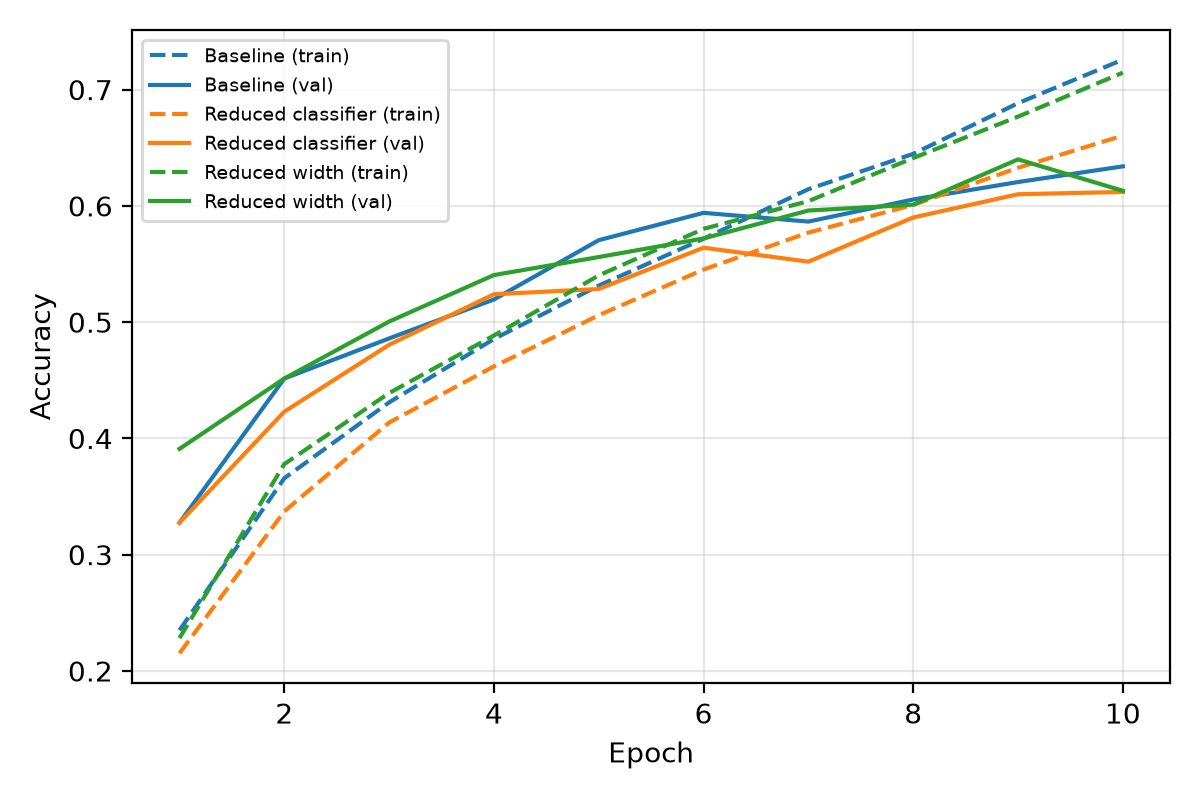
\includegraphics[width=0.44\linewidth]{plot_accuracy.png}
\hfill
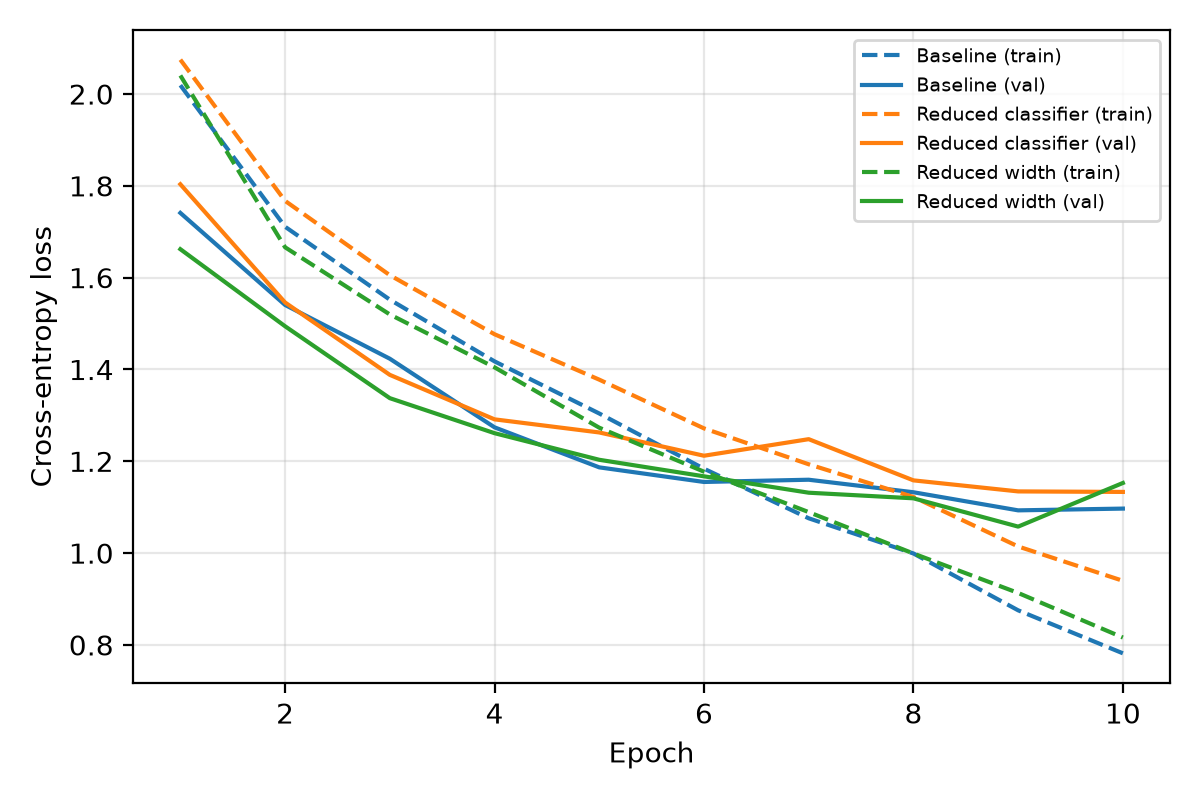
\includegraphics[width=0.44\linewidth]{plot_loss.png}
\caption{Training (dashed) and validation (solid) accuracy and loss versus epoch. Training curves are running values with dropout on.}
\end{figure}

\begin{figure}[H]
\centering
\begin{minipage}[c]{0.44\linewidth}
\centering
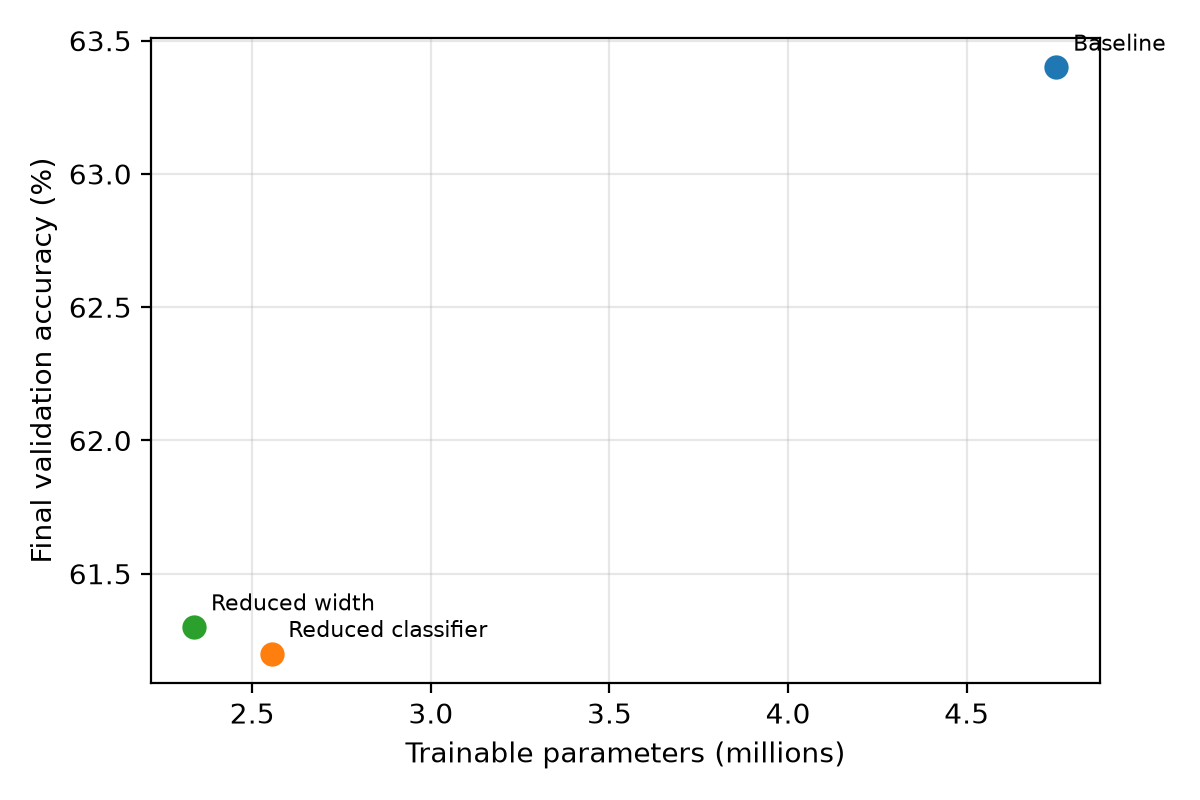
\includegraphics[width=\linewidth]{plot_params.png}
\end{minipage}
\hfill
\begin{minipage}[c]{0.44\linewidth}
\centering
\small
\begin{tabular}{lrr}
\toprule
Model & MACs/image & Time \\
\midrule
Baseline & 161.0\,M & 100\% \\
Exp 2 & 158.8\,M & 100\% \\
Exp 3 & 43.8\,M & 37\% \\
\bottomrule
\end{tabular}
\end{minipage}
\caption{Left: validation accuracy versus trainable parameters. Right: analytically counted multiply-accumulates per image and measured time relative to the baseline.}
\end{figure}

\section*{Analysis}

\textbf{Experiment 1 (baseline).} Validation accuracy rose steadily from 32.8\% to 63.4\% and validation loss fell from 1.74 to about 1.10. The model is not underfitting, since it reaches 84\% training accuracy in evaluation mode, but the 20-point gap shows it fits the training set much better than unseen data. From epoch 6 the validation loss flattens (1.155, 1.160, 1.133, 1.093, 1.097) while the training loss keeps falling (1.18 to 0.78), which is the start of overfitting rather than a clear rise in validation loss. The model has not fully converged in 10 epochs: training loss is still dropping by about 0.1 per epoch and validation accuracy was still improving at epoch 10. Stable but still improving is the fairest description.

\textbf{Experiment 2 (classifier size).} Reducing the head from 512-256 to 256-128 removes 46\% of the parameters (4.75M to 2.55M) because the first FC layer alone held 4.19M weights, 88\% of the baseline. Validation accuracy fell by 2.2 points (63.4\% to 61.2\%), the training accuracy fell by 7.9 points and the gap shrank from 20.3 to 14.6 points. Most of what was removed was therefore capacity to fit the training data, not capacity that helps on new data, so the classifier contributes mostly memorisation capacity here. The loss curve of Exp 2 was also still falling at epoch 10, so a part of the lower accuracy may be slower convergence. Training time did not change (444 s versus 445 s) because the FC layers account for only about 3\% of the arithmetic.

\textbf{Experiment 3 (convolutional width).} Halving the filters cuts the conv parameters by 75\% (423k to 106k) and the total by 51\%, but reduces the multiply-accumulates per image by 73\% (161M to 44M) because a conv weight is reused at every spatial position. Measured training time fell by 63\% (445 s to 164 s, 2.7 times faster), a little less than the arithmetic count suggests since the FC layers and data handling do not shrink. Validation accuracy was 2.1 points lower (61.3\%) and the training accuracy 3.1 points lower, with a gap of 19.3 points, close to the baseline. So the narrow model still overfits, because it kept the large first FC layer (2.1M weights), while losing a little accuracy for a large saving in compute.

\textbf{Complexity versus cost.} Exp 2 and Exp 3 have similar parameter counts (2.55M and 2.34M) but very different cost, so parameters measure memory, while the convolutions decide the running time. Figure 2 (left) alone would hide this. The reduced-width model gives the best accuracy per unit of compute.

\textbf{Caveats.} Each model was trained once. Validation accuracy on 2\,000 images has a standard error of about 1 point, and the value can move by more than that between epochs (the Exp 3 validation accuracy dropped from 64.0\% at epoch 9 to 61.3\% at epoch 10). The 2-point differences between models are therefore suggestive, not conclusive. The test accuracies (62.5\%, 62.0\%, 63.3\%) are similarly close and even reverse the validation ordering, which is why they were not used for the comparison. The images were a JPEG copy of CIFAR-10.

\section*{Proposed modification (not trained)}
\textbf{Add batch normalisation after every convolution} (before the ReLU), in particular in the reduced-width model. For each channel it computes $\hat x=(x-\mu_B)/\sqrt{\sigma_B^2+\epsilon}$ and outputs $\gamma\hat x+\beta$, with $\mu_B,\sigma_B^2$ taken over the mini-batch. It adds only $2\times(16+32+64+64+64)=480$ parameters and a small amount of extra arithmetic compared with 44M multiply-accumulates. \textbf{Expected effect:} the baseline had not converged in 10 epochs, and normalised activations usually allow faster optimisation at the same learning rate, so the narrow network should reach a higher validation accuracy within the same budget, recovering the 2-point loss while keeping the 63\% time saving. Batch statistics also add a mild regularising noise that may narrow the gap slightly. It would not fix the overfitting caused by the large first FC layer, and it makes correct use of \texttt{model.eval()} more important.

\end{document}
